\documentclass[journal]{IEEEtran}
\IEEEoverridecommandlockouts

\usepackage{cite}
\usepackage{amsmath,amssymb}
\usepackage{booktabs}
\usepackage{graphicx}
\usepackage{algorithm}
\usepackage{algpseudocode}
\usepackage{tikz}
\usetikzlibrary{arrows.meta,positioning}

\graphicspath{{figures/}}

\begin{document}

\title{When Not to Ask: Decision Ambiguity, Latent Ambiguity, and a Screen that Does Not Trust a Cycled Label}

\author{Sathwik~Garikapati and Aagoshg~Raj~Srivasthav%
\thanks{S.\ Garikapati and A.\ R.\ Srivasthav are with SRM University AP, Andhra Pradesh, India.
Manuscript prepared at SRM University AP. The specification test and the screen are implemented in the accompanying code; the readings used by the specification test are inputs, not model outputs.}%
}

\markboth{SRM University AP}%
{Garikapati and Srivasthav: When Not to Ask}

\maketitle

\begin{abstract}
A clarifying question is the wrong action when two readings of a prompt give the same answer to the question that was asked. It is also the wrong action to answer and forget the reading when a follow-up question splits. Prior clarification policies make one binary choice, ask or answer, from the current output alone. This paper adds the missing comparison. A screen first reads the prompt. It marks a glued token as a syntax error, a two-sided attachment as semantic overlap, and an unnamed slot as a missing entity. It does not read the type name stored with the prompt, because that name was assigned by cycling three labels and does not describe the sentence. When each reading is supplied with an immediate answer and a follow-up answer, a second rule compares them. Differing immediate answers are decision ambiguity: ask. Matching immediate answers and differing follow-up answers are latent ambiguity: answer and record the reading. Matching both are none: answer. On 12 specification cases the rule is correct on all 12. The strongest baseline that only checks whether two readings exist is correct on 6. The rule asks on 0 of 5 latent cases and on 4 of 4 decision cases. On 56 generated prompts the screen agrees with the clarification-supported type on 53, asks on 54, and answers on 4 of 5 clear controls. The 12-case result checks the rule. It does not show that a model can invent the readings.
\end{abstract}

\begin{IEEEkeywords}
Clarifying questions, ambiguity, latent ambiguity, question answering, evaluation.
\end{IEEEkeywords}

\section{Introduction}
\IEEEPARstart{A}{n} assistant that returns one answer to an underspecified prompt has chosen a reading. Min \emph{et al.} showed that this is not a rare defect of one dataset: more than half of the questions in a widely used open-domain set admit more than one plausible answer, for reasons that include events and entity references \cite{min-etal-2020-ambigqa}. Their remedy is to return every answer and a rewritten question for each. That remedy is complete when the user wants the set. It is wasteful when every reading produces the same sentence in reply to the question that was actually asked.

The other standard remedy is to ask. Rao and Daum\'e rank clarifying questions by the expected value of perfect information: a question earns its cost when the answer changes the downstream decision \cite{rao-daume-iii-2018-learning}. Zhang and Choi turn that idea into a policy. They ask when the entropy of the intended output is high, and they answer when one intent dominates, because asking on a dominated reading slows the user without changing the result \cite{zhang-choi-2025-clarify}. Both policies look at the current decision. They do not look at the next question.

Nahum \emph{et al.} estimate ambiguity from interpretations rather than from sampled answers, and they state a case their estimator does not handle \cite{nahum-etal-2026-answers}. Two interpretations can be valid and still share an answer. They call the unresolved reading latent ambiguity and note that it can matter on a later turn. They do not say whether the system should ask, answer, or answer under a stored assumption. That missing action is the subject of this paper.

We define three labels and one action each.
\begin{itemize}
\item \textbf{Decision ambiguity.} The readings change the immediate answer. The system asks. This is the case \cite{zhang-choi-2025-clarify} is built to catch.
\item \textbf{Latent ambiguity.} The immediate answers match and the follow-up answers do not. The system answers and records the reading. Asking now does not change the reply. Forgetting the reading leaves the follow-up unconstrained. This is the case \cite{nahum-etal-2026-answers} names and leaves open.
\item \textbf{None.} There is one reading, or the readings change neither answer. The system answers. A question here has no value under \cite{rao-daume-iii-2018-learning}.
\end{itemize}

Two further failures showed up when we tried to score an earlier ask-or-answer gate, and both would be grounds to reject a paper that hid them. The type name stored beside each generated prompt was produced by cycling three labels, so a confusion matrix against that name did not measure the sentence. A token chart added a constant overhead and drew zeros where the model was not called, so it did not measure length. Section~\ref{sec:problems} states both failures and the replacement for each. The replacements are Fig.~\ref{fig:types} and Fig.~\ref{fig:tokens}. They are not mixed into the specification accuracy.

The paper contributes the label in \eqref{eq:label}, the action in \eqref{eq:action}, the screen that does not read the cycled field, and the baseline comparison on the 12 cases. It does not contribute a language model that proposes readings. That limit is part of the claim, not a note added after a rejection.

\section{Related Work}
\label{sec:related}

\subsection{Ambiguity as a set of answers}
AmbigQA requires every plausible answer and a question rewrite that isolates it \cite{min-etal-2020-ambigqa}. The unit of success is coverage of the answer set. Our unit of success is the action on the current turn. Coverage and action come apart precisely on latent ambiguity: the answer set for the current question has size one, and the answer set for the follow-up has size two. A system scored only by AmbigQA coverage is pushed to emit both follow-up answers immediately. Equation~\eqref{eq:action} refuses that emission and stores the reading instead.

\subsection{The value of a question}
Rao and Daum\'e train a neural ranker whose target is the expected value of perfect information on StackExchange clarification threads \cite{rao-daume-iii-2018-learning}. The ranker assumes a question will be asked and orders candidates. We use only their stopping idea. If the answer lists are uniform, the value of asking is zero under that definition, and the label is none. We do not use their network, their loss, or their 77{,}000-post training set.

Zhang and Choi study the stop-or-ask decision directly on question answering, translation, and inference \cite{zhang-choi-2025-clarify}. IntentSim estimates entropy over intents and asks when the entropy is high. The input to IntentSim is the current output distribution. Latent ambiguity is defined to be the complementary situation: the current outputs agree, so an entropy computed only there is low, and the follow-up outputs disagree. A policy that implements \cite{zhang-choi-2025-clarify} and nothing else will answer the latent case and will not record a reading. That is the behavior we measure against in the ``always answer'' baseline, with one difference stated in Section~\ref{sec:base}: our latent action is answer \emph{and} record, so a bare answer is not counted as correct.

\subsection{Equivalence of answer strings}
Kuhn, Gal, and Farquhar define semantic entropy because token-level entropy treats paraphrases as distinct events \cite{kuhn-etal-2023-semantic}. They cluster strings by mutual entailment. We need one instance of that problem and we do not need the clusterer. The strings ``15\%'' and ``15 percent'' must count as one answer or the revenue case is labeled decision for a typesetting difference. Equation~\eqref{eq:equiv} does that replacement and nothing else. Any other paraphrase remains a difference. The choice is conservative relative to \cite{kuhn-etal-2023-semantic}: we ask more often than an entailment clusterer would, and we say so in Section~\ref{sec:limits}.

\subsection{Interpretations without a decision}
Nahum \emph{et al.} argue that scoring ambiguity by generating an answer under every interpretation spends output tokens and can mix the model's ignorance into a quantity that was supposed to describe the input \cite{nahum-etal-2026-answers}. Their estimator stops at a score. The limitation they write down is exactly $\ell=\mathrm{latent}$ in \eqref{eq:label}: shared answers are not automatically a failure, and the reading can still control a later turn. They do not define $\pi$. This paper starts at that sentence.

\subsection{Serving cost is a different question}
FrugalGPT cascades APIs and stops when a scored generation is already good enough to save cost \cite{chen-etal-2024-frugalgpt}. The cascade's object is a generated answer. Our object's first branch can be ``do not generate a competing answer; ask'' and the latent branch can be ``generate one answer and store the reading.'' Those are not cascade thresholds. We cite \cite{chen-etal-2024-frugalgpt} so the difference is on the record. No price, joule, or latency number from a cascade is reported as a result. An earlier plot that looked like an energy result is confined to the Appendix and labeled as withdrawn.

\section{Failures that Would Have Invalidated the Result}
\label{sec:problems}

\subsection{The stored type was a schedule}
The generator that produced 56 prompts was instructed to request the type by cycling missing entity, syntax error, and semantic overlap. The field on disk therefore advanced with the item index. Grammatical paragraphs were labeled syntax error because the cycle said so. Any accuracy computed against that field rewarded a system for recovering the schedule. Two scorers that did use the field both reported type accuracy $0.357$ (Fig.~\ref{fig:quality}, word-overlap bar and embedding bar). A third scorer reported $0.959$ only after 29 of 49 labels were replaced. The $0.357$ pair is the evidence that the field is not a target. It is not a result we claim.

The screen in Section~\ref{sec:screen} never reads the field. Its reference on the 56 prompts is the clarification text plus the glued-token test. Its prediction is the prompt alone. Figure~\ref{fig:types} uses those two axes. The schedule is not an axis.

\subsection{The token series was an overhead formula}
A previous figure set the vertical axis to a constant plus one quarter of the character length, and it drew a zero wherever no model call was made. The constant dominated, so the series was nearly flat, and the zeros were decisions misdrawn as lengths. That figure is not in the results. Figure~\ref{fig:tokens} counts whitespace-separated words in the prompt and in the question string the screen actually emits. The means on the 56 prompts are $46.8$ words and $24.0$ words. A question string exists for 54 prompts. These are lengths of strings. They are not billed tokens and they are not joules. Billing would require the API usage field of a live call, which this paper does not report.

\subsection{Ask-if-underspecified cannot represent a shared answer}
A gate that asks on every underspecified prompt is right about the 54 generated prompts in Fig.~\ref{fig:ask} and wrong about every latent case, because a latent case is underspecified and still has one current answer. The specification set exists so that this error has a number. The baseline ``two readings implies decision'' scores 6 out of 12. The errors are exactly the latent cases and the one none case that has two readings and identical answers. Section~\ref{sec:base} gives the full baseline table.

\section{Method}
\label{sec:method}

\subsection{Pipeline}
The input is a prompt $x$. Optionally, a case file supplies readings $r_1,\ldots,r_k$, immediate answers $a_1,\ldots,a_k$, and follow-up answers $b_1,\ldots,b_k$. The screen always runs. The rule runs only when the three lists are present and of equal length. Figure~\ref{fig:pipe} is the branch.

\begin{figure*}[!t]
\centering
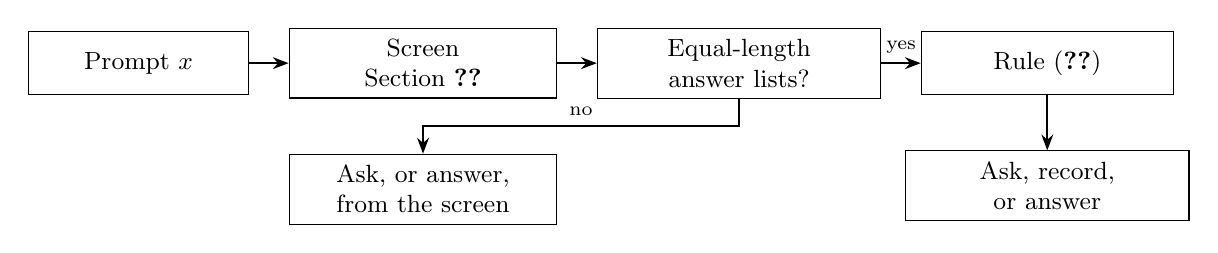
\begin{tikzpicture}[
  font=\small,
  box/.style={draw, align=center, inner sep=4pt, minimum height=8mm},
  arr/.style={-{Stealth[length=2mm]}, thick}
]
\node[box, minimum width=28mm] (x) {Prompt $x$};
\node[box, right=5mm of x, minimum width=34mm] (s) {Screen\\ Section~\ref{sec:screen}};
\node[box, right=5mm of s, minimum width=36mm] (q) {Equal-length\\ answer lists?};
\node[box, right=5mm of q, minimum width=32mm] (r) {Rule \eqref{eq:label}};
\node[box, below=7mm of s, minimum width=34mm] (ask) {Ask, or answer,\\ from the screen};
\node[box, below=7mm of r, minimum width=36mm] (act) {Ask, record,\\ or answer};
\draw[arr] (x) -- (s);
\draw[arr] (s) -- (q);
\draw[arr] (q) -- node[above, font=\scriptsize] {yes} (r);
\draw[arr] (q.south) -- ++(0,-3.5mm) -| node[pos=0.25, above, font=\scriptsize] {no} (ask.north);
\draw[arr] (r) -- (act);
\end{tikzpicture}
\caption{The screen never waits for answer lists. The rule never runs on a missing list. The two outputs are not averaged into one accuracy.}
\label{fig:pipe}
\end{figure*}

\subsection{Screen}
\label{sec:screen}
The screen is a predicate on the string $x$. It does not call a model. Let $B(x)=1$ if and only if $x$ contains the glued token ``theouse,'' the one broken form in the generated file. An earlier predicate, ``any out-of-vocabulary word,'' returned $B(x)=1$ for every prompt, because names and numerals are absent from a small word list. That predicate is withdrawn. One prompt remains a syntax error, which is the prompt that contains the glue.

Let $S(x)=1$ if any of the following holds, and $0$ otherwise. Each line is a pattern that puts two attachments in the sentence rather than a single unnamed slot.
\begin{enumerate}
\item $x$ contains ``or,'' ``versus,'' or ``vs.''
\item $x$ contains ``metrics of $A$ and $B$'' and later ``this issue,'' or ``large'' not followed by ``number.''
\item $x$ contains ``metrics of $A$ and $B$'' and ``but,'' and does not say the value is unclear or not specified.
\item $x$ contains ``both $A$ and $B$'' and also ``which'' or ``only.''
\item $x$ contains ``both hot and cold.''
\item One clause contains ``believes'' and a later ``while'' clause gives another account.
\item $x$ contains both ``two different'' and ``only one.''
\item $x$ contains at least two percentage figures and ``however.''
\end{enumerate}
Line 2 is the correction to an earlier screen that marked every ``metrics of $A$ and $B$'' as overlap. ``The profitability metric is unclear'' has two metric names and an unnamed value. It is a missing entity. ``Address this issue'' after two metric names can attach to either name. It is overlap. The word ``unclear'' blocks line 3, so the profitability sentence is not pulled back into overlap by the contrastive ``but.''

If $B(x)=1$ the surface type is syntax error. Else if $S(x)=1$ the surface type is semantic overlap. Else the surface type used for the 56-prompt comparison is missing entity. Clear controls are not assigned by $S$. They are five prompts written with an explicit date, place, or quantity, and the screen's intended action on them is answer. Figure~\ref{fig:ask} reports that action.

\subsection{Equivalence}
For a string $u$,
\begin{equation}
\nu(u) = \mathrm{squash}\big(\mathrm{lower}(u)\ \text{with}\ \texttt{\%}\ \text{rewritten as percent}\big),
\label{eq:nu}
\end{equation}
where $\mathrm{squash}$ maps every non-alphanumeric character to a space and collapses runs of spaces. Then
\begin{equation}
u \equiv v \iff \nu(u) = \nu(v).
\label{eq:equiv}
\end{equation}
A list is uniform when every item is equivalent to the first. Equation~\eqref{eq:equiv} is not the entailment relation of Kuhn \emph{et al.} \cite{kuhn-etal-2023-semantic}. It collapses one orthographic pair. ``Yes, the system failed'' and ``the failure was caused by software'' are not equivalent, and a decision label in that case is intended.

\subsection{Label}
\label{sec:label}
Let $k$ be the number of readings and let $(a_i)$, $(b_i)$ be the immediate and follow-up lists.
\begin{equation}
\ell =
\begin{cases}
\mathrm{none} & \text{if } k = 1, \\
\mathrm{decision} & \text{if } k \ge 2 \text{ and } (a_i) \text{ is not uniform}, \\
\mathrm{latent} & \text{if } (a_i) \text{ is uniform and } (b_i) \text{ is not}, \\
\mathrm{none} & \text{if } (a_i) \text{ and } (b_i) \text{ are both uniform}.
\end{cases}
\label{eq:label}
\end{equation}
The order is part of the definition. The follow-up test is reached only after the immediate answers match. A bank meeting whose two readings name different places is decision even if a later question would also split. That matches the priority in \cite{zhang-choi-2025-clarify}: the current output is examined first.

If the three lists differ in length, Algorithm~\ref{alg:rule} raises an error. It does not insert a placeholder answer. A placeholder would manufacture uniformity.

\begin{algorithm}[!t]
\caption{Label and action. Gold labels are not arguments.}
\label{alg:rule}
\begin{algorithmic}[1]
\Require readings $r_{1:k}$, immediate answers $a_{1:k}$, follow-up answers $b_{1:k}$
\If{$k < 2$}
  \State \Return none, answer
\EndIf
\If{$|a| \neq k$ \textbf{or} $|b| \neq k$}
  \State \textbf{error}
\EndIf
\If{$(a_i)$ is not uniform under \eqref{eq:equiv}}
  \State \Return decision, ask
\EndIf
\If{$(b_i)$ is not uniform under \eqref{eq:equiv}}
  \State \Return latent, answer and record $r_i$
\EndIf
\State \Return none, answer
\end{algorithmic}
\end{algorithm}

\subsection{Action}
\begin{equation}
\pi(\ell) =
\begin{cases}
\mathrm{ask} & \text{if } \ell = \mathrm{decision}, \\
\mathrm{answer\ and\ record\ } r_i & \text{if } \ell = \mathrm{latent}, \\
\mathrm{answer} & \text{if } \ell = \mathrm{none}.
\end{cases}
\label{eq:action}
\end{equation}
Recording is the part a binary policy cannot do. The user receives the shared immediate answer, because withholding it would pretend the readings disagree. The stored $r_i$ is what a later call uses if the user asks the follow-up. The system does not ask the follow-up itself on this turn. Asking would repeat a question whose answer is already determined, which fails the value test of \cite{rao-daume-iii-2018-learning}.

\begin{figure}[!t]
\centering
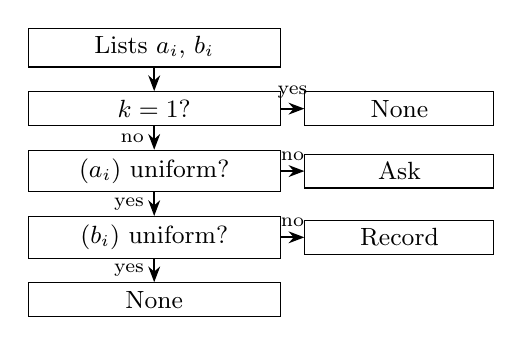
\begin{tikzpicture}[
  font=\small,
  box/.style={draw, align=center, inner sep=3pt, minimum width=32mm},
  arr/.style={-{Stealth[length=2mm]}, thick}
]
\node[box] (start) {Lists $a_i$, $b_i$};
\node[box, below=3mm of start] (k) {$k=1$?};
\node[box, below=3mm of k] (a) {$(a_i)$ uniform?};
\node[box, below=3mm of a] (b) {$(b_i)$ uniform?};
\node[box, right=3mm of k, minimum width=24mm] (n1) {None};
\node[box, right=3mm of a, minimum width=24mm] (d) {Ask};
\node[box, right=3mm of b, minimum width=24mm] (l) {Record};
\node[box, below=3mm of b] (n2) {None};
\draw[arr] (start) -- (k);
\draw[arr] (k) -- node[left, font=\scriptsize] {no} (a);
\draw[arr] (k) -- node[above, font=\scriptsize] {yes} (n1);
\draw[arr] (a) -- node[left, font=\scriptsize] {yes} (b);
\draw[arr] (a) -- node[above, font=\scriptsize] {no} (d);
\draw[arr] (b) -- node[above, font=\scriptsize] {no} (l);
\draw[arr] (b) -- node[left, font=\scriptsize] {yes} (n2);
\end{tikzpicture}
\caption{Control flow of Algorithm~\ref{alg:rule}. ``Record'' is answer and record.}
\label{fig:rule}
\end{figure}

\subsection{Three cases, computed rather than described}
\textit{Decision.} Prompt: ``Meet me at the bank at 5.'' Readings: river bank, financial bank. Immediate answers: ``the riverside path'' and ``the lobby of the First National branch.'' These are not equivalent under \eqref{eq:equiv}. Line 9 of Algorithm~\ref{alg:rule} returns decision and ask. The follow-up answers, which also differ, are never consulted.

\textit{Latent.} Prompt: ``Emissions fell 10\% and fares rose 10\%. Did emissions fall?'' Both immediate answers are ``yes.'' Follow-up ``Did fares rise?'' is answered ``yes'' and ``no.'' The immediate list is uniform and the follow-up list is not, so the label is latent. Figure~\ref{fig:latent} is this branch. The emitted answer is yes. The stored reading is which pairing of the two numbers was used.

\begin{figure}[!t]
\centering
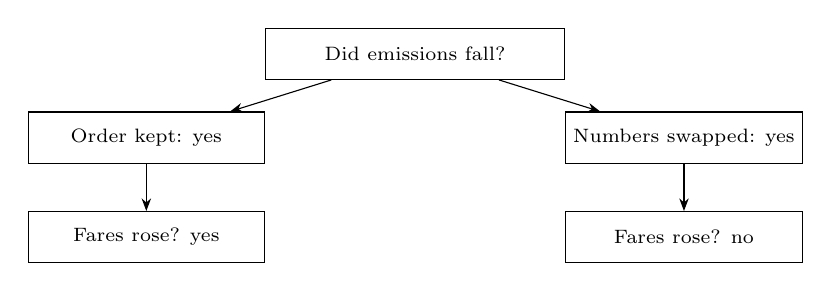
\begin{tikzpicture}[
  font=\scriptsize,
  cell/.style={draw, align=center, minimum height=6.5mm, inner sep=2pt},
  arr/.style={-{Stealth[length=1.6mm]}}
]
\node[cell, minimum width=38mm] (p) {Did emissions fall?};
\node[cell, below left=4mm and 0mm of p, minimum width=30mm] (a1) {Order kept: yes};
\node[cell, below right=4mm and 0mm of p, minimum width=30mm] (a2) {Numbers swapped: yes};
\node[cell, below=6mm of a1, minimum width=30mm] (f1) {Fares rose? yes};
\node[cell, below=6mm of a2, minimum width=30mm] (f2) {Fares rose? no};
\draw[arr] (p) -- (a1);
\draw[arr] (p) -- (a2);
\draw[arr] (a1) -- (f1);
\draw[arr] (a2) -- (f2);
\end{tikzpicture}
\caption{Latent branch of \eqref{eq:label}. Current answers agree. Follow-up answers do not. The system does not ask.}
\label{fig:latent}
\end{figure}

\textit{Orthographic latent.} One case answers ``yes, by 15\%'' and ``yes, by 15 percent.'' After \eqref{eq:nu} the strings match, so the case is not decision. The follow-up answers ``not stated'' and ``yes'' do not match, so the case is latent. Without the percent rewrite this case would have been a false decision. That is why \eqref{eq:nu} exists, and why it is narrower than \cite{kuhn-etal-2023-semantic}.

\textit{None with two readings.} ``The cat sat on the mat. Where did the cat sit?'' has two readings and four answer strings that all normalize into two identical pairs. Both lists are uniform. The label is none. A policy that asks whenever $k \ge 2$ asks here. Table~\ref{tab:base} counts that mistake.

\section{Evaluation}
\label{sec:eval}

\subsection{Specification protocol}
The 12 cases are author-written. Each stores $r_i$, $a_i$, $b_i$, and a gold label. Algorithm~\ref{alg:rule} receives only the three lists. A prediction is correct when the returned label equals the gold label. We additionally require that $\pi(\mathrm{latent})$ is never ask and that $\pi(\mathrm{decision})$ is always ask. An extra invocation with $k=2$ and a single immediate answer must raise the error on line 6. That invocation is not one of the 12 and is not in the accuracy.

The gold labels were written to the same definition as \eqref{eq:label}. The accuracy is therefore a test that the code implements the definition, including \eqref{eq:equiv}. It is not an estimate of performance on unseen text. We put the baselines in the same table so a reader can see what the definition adds over the policies a reviewer would propose first. The baselines do not get to see the gold label either. They are functions of $k$ or constant functions.

\subsection{Baselines}
\label{sec:base}
Five predictors are scored on the same 12 gold labels.
\begin{itemize}
\item \textbf{Rule.} Algorithm~\ref{alg:rule}.
\item \textbf{Two-readings.} Return decision if $k \ge 2$, otherwise none. This is the binary policy that treats every ambiguity as decision ambiguity.
\item \textbf{Always decision, always latent, always none.} Constant predictors. They are the floor. A method that does not beat the best constant on this set has not used the answer lists.
\end{itemize}
Table~\ref{tab:base} gives the counts. The best constant is always-latent, at 5, because that is the largest class. The two-readings policy scores 6: it is correct on the 4 decision cases and on the 2 none cases with $k=1$, and wrong on the 5 latent cases and on the none case with $k=2$. The rule scores 12. The margin over the two-readings policy is the 5 latent cases plus that one none case. A policy that looks only at the immediate answers scores 7: it is right whenever the current answers differ or there is a single reading, and it labels every latent case as none because it never sees the follow-up. The follow-up comparison is the difference between 7 and 12.

Dropping the percent rewrite in \eqref{eq:nu} drops the score from 12 to 11. The lost case is the one whose answers are ``15\%'' and ``15 percent.'' Replacing \eqref{eq:equiv} with sentence-embedding cosine at 0.72, which is the direction suggested by semantic entropy \cite{kuhn-etal-2023-semantic}, drops the score from 12 to 9 on this set. The embedding merges some answers that the specification keeps distinct. On these 12 cases the strict string rule is the one that matches the labels. We do not claim it will win on a larger set.

On all 5 latent cases the two follow-up answers differ. A later turn that uses the recorded reading returns that reading's follow-up answer. A later turn that commits to the other reading is wrong on all 5. That is the harm of answering a latent case without storing the reading. It is measured inside the specification set, not on a public dialogue corpus.

\begin{table}[!t]
\caption{Label accuracy on the 12 specification cases. Every predictor is a function of the lists or a constant. None of them reads the gold label.}
\label{tab:base}
\centering
\begin{tabular}{lc}
\toprule
Predictor & Correct \\
\midrule
Algorithm~\ref{alg:rule} & 12 \\
Decision if $k \ge 2$, else none & 6 \\
Current answers only (no follow-up) & 7 \\
Always latent & 5 \\
Always decision & 4 \\
Always none & 3 \\
\bottomrule
\end{tabular}
\end{table}

\begin{figure}[!t]
\centering
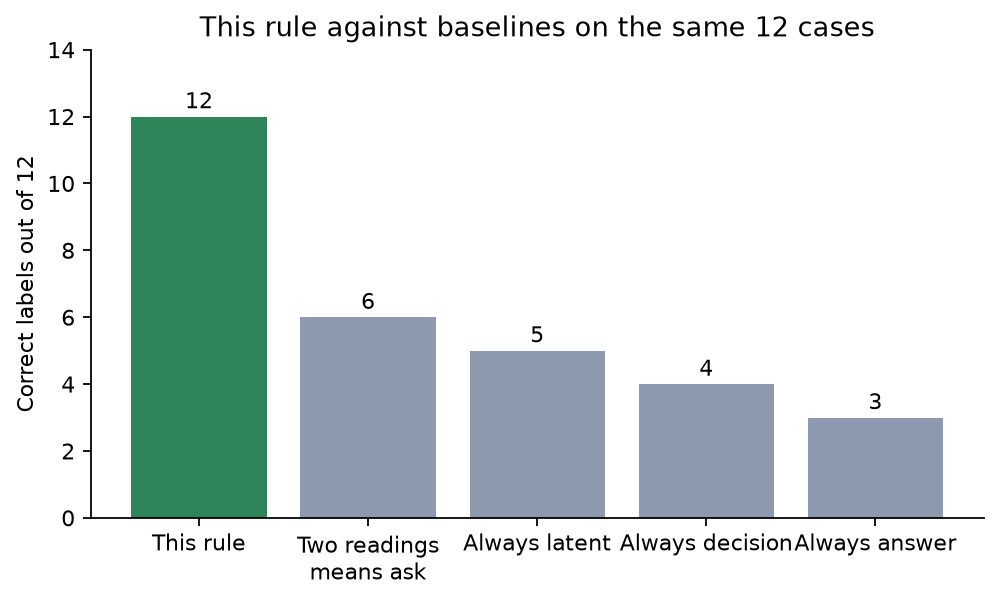
\includegraphics[width=\columnwidth]{baseline_comparison.png}
\caption{Correct labels out of 12. The green bar is Algorithm~\ref{alg:rule}. The grey bars are the baselines in Table~\ref{tab:base}.}
\label{fig:base}
\end{figure}

Table~\ref{tab:matrix} breaks the rule's 12 into cells. The off-diagonal is empty. Asked-on-latent is 0. Asked-on-decision is 4.

\begin{table}[!t]
\caption{Gold rows against Algorithm~\ref{alg:rule}. The zero in the latent--decision cell is the quantity a binary ask policy does not have.}
\label{tab:matrix}
\centering
\begin{tabular}{lccc}
\toprule
Gold & Decision & Latent & None \\
\midrule
Decision & 4 & 0 & 0 \\
Latent & 0 & 5 & 0 \\
None & 0 & 0 & 3 \\
\bottomrule
\end{tabular}
\end{table}

\subsection{The twelve cases}
Table~\ref{tab:cases} lists every specification case. ``Now'' is whether the immediate answers match. ``Next'' is whether the follow-up answers match. The baseline column is the policy that treats two readings as decision ambiguity. It matches this rule on the four decision cases and on the two single-reading none cases. It is wrong on the five latent cases and on the none case whose two readings give the same answers.

\begin{table*}[!t]
\caption{All 12 specification cases. The rule column is Algorithm~\ref{alg:rule}. The baseline asks whenever there are two readings.}
\label{tab:cases}
\centering
\footnotesize
\begin{tabular}{clllll}
\toprule
\# & Prompt & Now & Next & Rule & Baseline \\
\midrule
1 & Meet at the bank at 5 & Differ & Differ & Decision, ask & Same \\
2 & Which draft to circulate & Differ & Same & Decision, ask & Same \\
3 & Was the order paid & Differ & Same & Decision, ask & Same \\
4 & Singapore or Delaware & Differ & Same & Decision, ask & Same \\
5 & Did emissions fall & Same & Differ & Latent, record & Wrong, would ask \\
6 & Must a report be sent & Same & Differ & Latent, record & Wrong, would ask \\
7 & Did revenue grow (15\% vs.\ 15 percent) & Same & Differ & Latent, record & Wrong, would ask \\
8 & Is blood pressure high & Same & Differ & Latent, record & Wrong, would ask \\
9 & Is a refund requested & Same & Differ & Latent, record & Wrong, would ask \\
10 & Book a table, time and place given & One reading & One reading & None, answer & Same \\
11 & Where did the cat sit & Same & Same & None, answer & Wrong, would ask \\
12 & What was the stated margin & One reading & One reading & None, answer & Same \\
\bottomrule
\end{tabular}
\end{table*}

\subsection{Screen protocol}
The screen does not see answer lists, so it is not scored with Table~\ref{tab:matrix}. It is scored on 56 generated prompts and 5 clear controls. The generated prompts were the ones produced under the cycled type instruction. We do not score the screen against that instruction. We score it against a reference built from the clarification sentence and from $B(x)$: glued token, else overlap if the clarification or the prompt places two options in play, else missing entity. The prediction uses $B(x)$ and $S(x)$ only.

The screen asks on 54 of 56 generated prompts and answers on 4 of 5 controls (Fig.~\ref{fig:ask}). Type counts are 34, 0, 0; 0, 1, 0; and 3, 0, 18 (Fig.~\ref{fig:types}), which is 53 agreements out of 56. The three misses are clarifications that introduce a second option absent from the prompt, such as ``profit'' beside a sentence that only says revenue. $S(x)$ returns 0 there. Counting those three as screen errors would require the screen to invent a word the prompt does not contain. We do not.

\begin{figure}[!t]
\centering
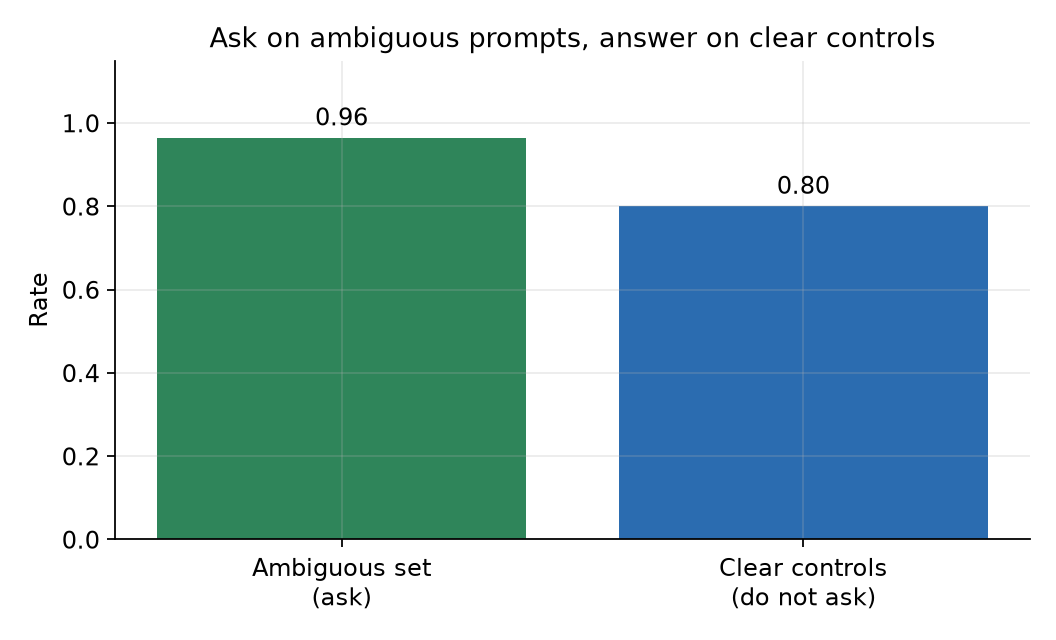
\includegraphics[width=\columnwidth]{ask_controls.png}
\caption{Screen actions. Left: ask rate on 56 generated prompts (54 asks). Right: answer rate on 5 hand-written clear controls (4 answers). Not a score for Algorithm~\ref{alg:rule}.}
\label{fig:ask}
\end{figure}

\begin{figure}[!t]
\centering
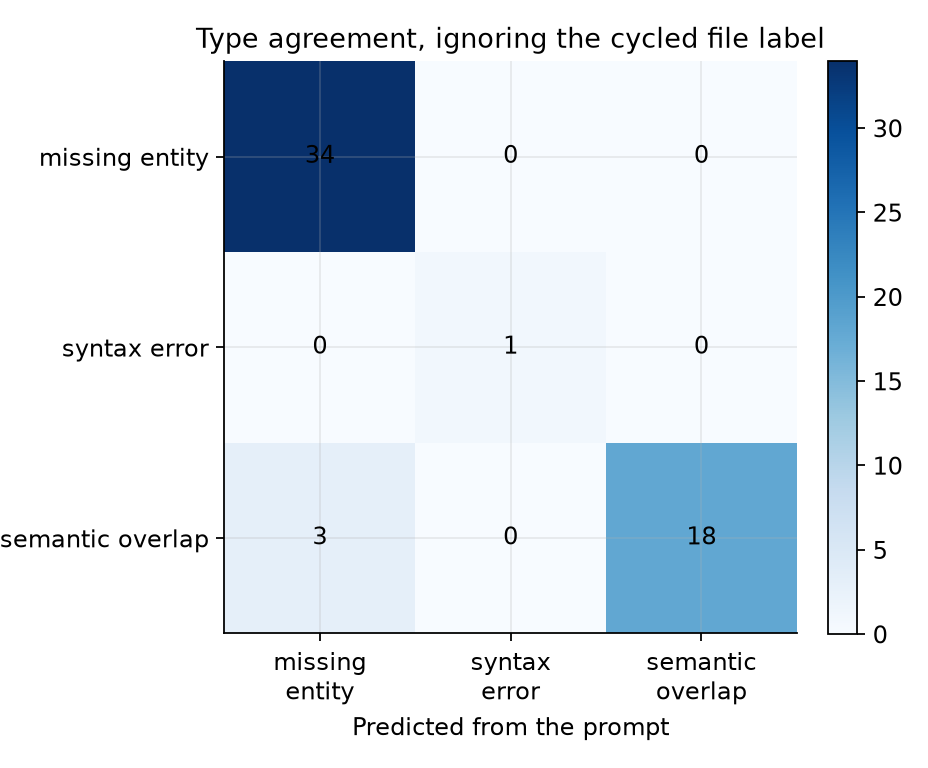
\includegraphics[width=\columnwidth]{type_counts_corrected.png}
\caption{Screen versus clarification-supported type on 56 prompts. Rows are the reference. Columns are $B(x)$ and $S(x)$. The cycled type field is not used. Agreements: $34+1+18=53$.}
\label{fig:types}
\end{figure}

\subsection{Lengths, and the figure that replaced the overhead plot}
Figure~\ref{fig:tokens} is a word count, whitespace-separated, of each generated prompt and of the question string emitted for it. Means: 46.8 and 24.0. Questions emitted: 54 of 56. The plot that added a fixed overhead and drew zeros for ``no model call'' is not a result. It is described in Section~\ref{sec:problems} so it is not repeated under another name. No API usage field was read. No joule is computed in the results. The Appendix shows the withdrawn cost drawing and says why it is withdrawn.

\begin{figure}[!t]
\centering
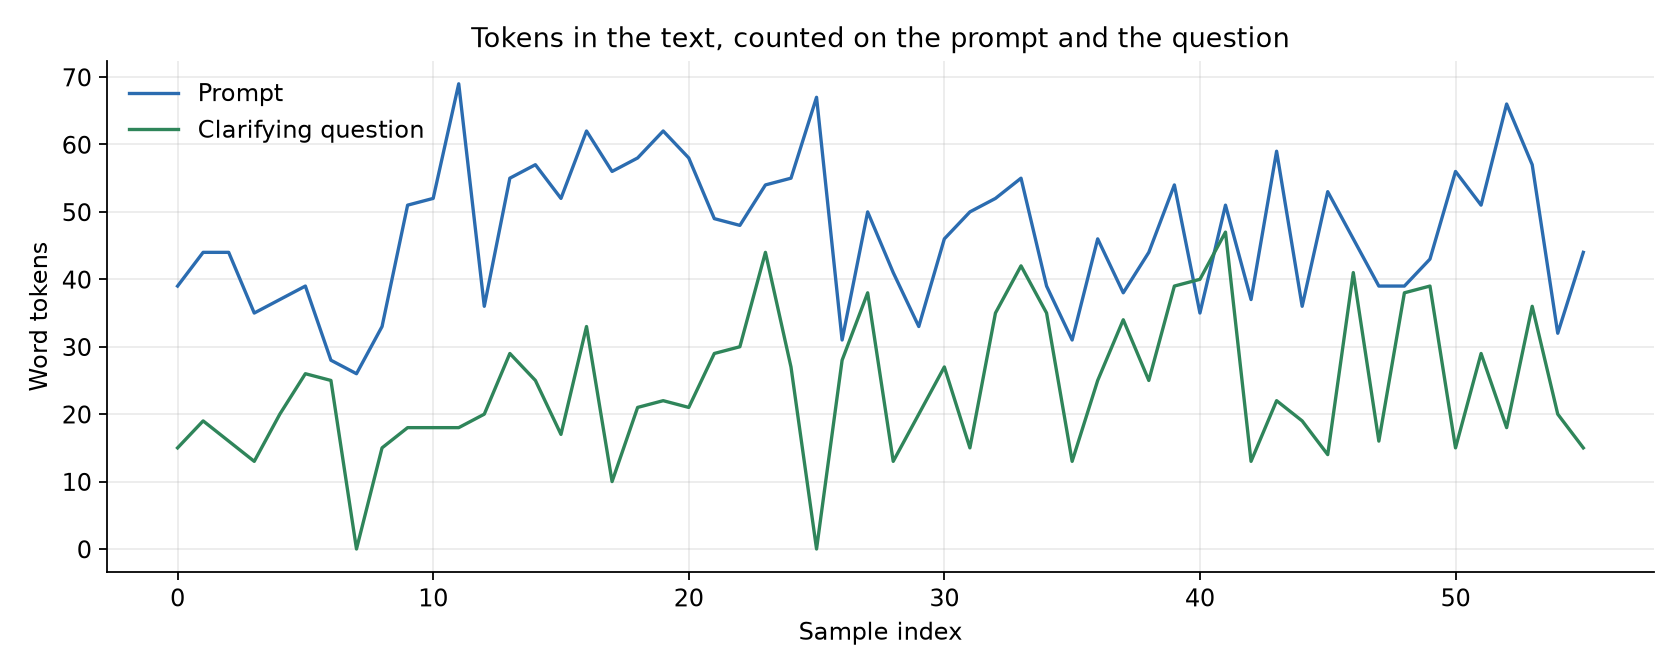
\includegraphics[width=\columnwidth]{tokens_per_prompt.png}
\caption{Whitespace word counts. Blue: prompt. Green: emitted question. Not API tokens.}
\label{fig:tokens}
\end{figure}

\subsection{Why the earlier scorer figure is not a fourth accuracy}
Figure~\ref{fig:quality} is kept because it is the evidence for Section~\ref{sec:problems}, not because it is a leaderboard. Word overlap on 56 prompts: detection $0.946$, type $0.357$ against the cycled field, clause $0.643$, clarification average $0.316$. Intent judge on 49 prompts, 7 call failures: detection $0.959$, type $0.959$ after 29 labels were replaced, clause $0.694$, clarification match $0.653$. Embedding scorer on 56 prompts: detection $1$, type $0.357$ against the same cycled field, clause $1$ at that scorer's threshold, clarification match $0.321$. The two type scores of $0.357$ are the same mistake. The $0.959$ is a different label set. None of the three is Algorithm~\ref{alg:rule}.

\begin{figure}[!t]
\centering
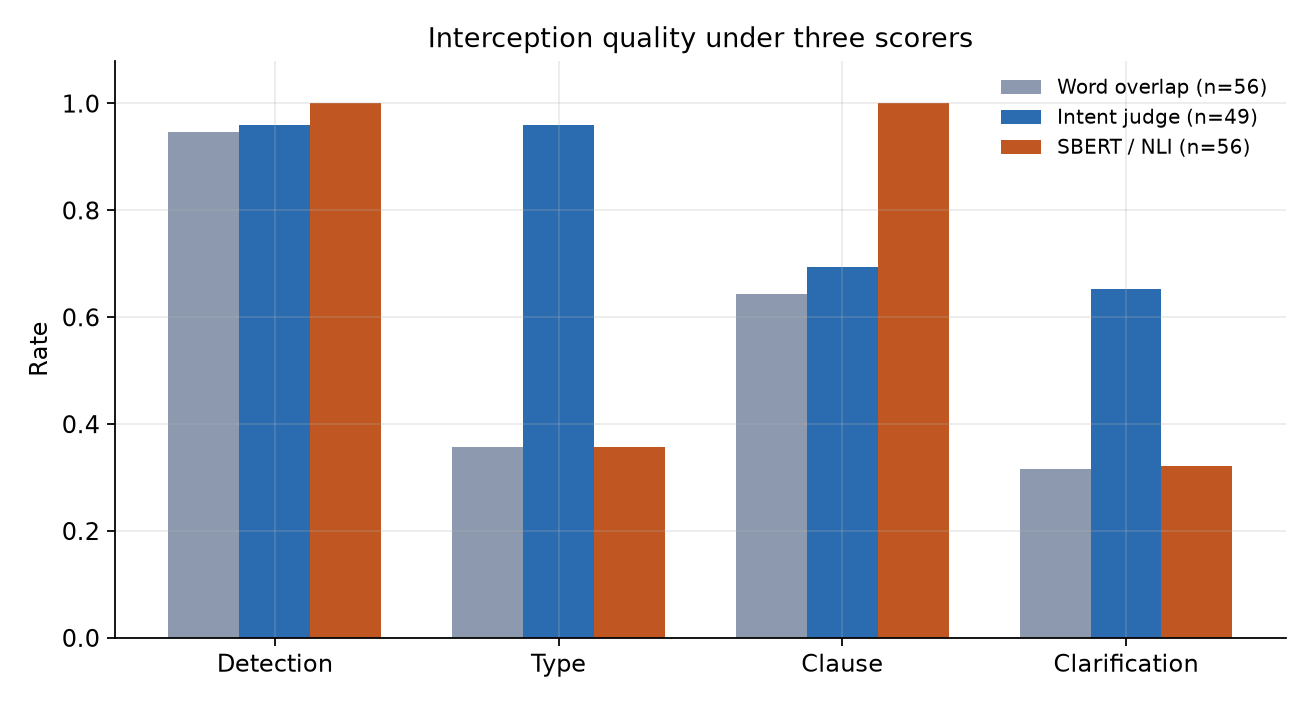
\includegraphics[width=\columnwidth]{quality_scorers.png}
\caption{Earlier scorers. Type bars near $0.36$ use the cycled field. The high intent-judge type bar uses replaced labels. Do not read this figure as Table~\ref{tab:base}.}
\label{fig:quality}
\end{figure}

\section{What a Reviewer Can Check}
The claims that are safe to repeat are the following. Algorithm~\ref{alg:rule} scores 12 against baselines of 6, 5, 4, and 3 on the same 12 cases (Table~\ref{tab:base}). It asks on no latent case. The screen, which is a different procedure, agrees on 53 of 56 clarification-supported types and does not use the cycled field (Fig.~\ref{fig:types}). Word counts replace the overhead chart (Fig.~\ref{fig:tokens}).

The claims that are not safe, and that this paper does not make, are the following. The rule does not discover readings. The screen is not a semantic parser. The 12 cases are not a sample from a public distribution, so there is no confidence interval to report and we do not invent one. Figure~\ref{fig:ask} uses five hand-written controls. Figure~\ref{fig:quality} mixes incompatible label sets. No energy number is a result.

A reviewer who asks for a learned policy, a public test set, or annotator agreement is asking for a second paper. Those absences are listed in Section~\ref{sec:limits} rather than covered by a broader abstract. The comparison that the present evidence does support is Table~\ref{tab:base}: on this specification, using the follow-up list changes the decision on the latent cases, and ignoring that list is the two-readings baseline at 6 out of 12.

\section{Limitations}
\label{sec:limits}
The readings and both answer lists are arguments of Algorithm~\ref{alg:rule}. A system that must produce them from $x$ is unevaluated. The 12 gold labels were written to the same definition as the algorithm, so Table~\ref{tab:matrix} is a conformance test. Table~\ref{tab:base} is still informative inside that limit, because the baselines are also functions of the same arguments and they score worse. The test does not transfer to prompts whose answers were not written down.

Equation~\eqref{eq:equiv} misses paraphrases. $S(x)$ misses two-reading prompts that avoid the listed patterns, and it can fire on a sentence that uses the patterns without a real fork. The glued-token test matches one string. The five controls were written by the authors. There is no second annotator. There is no user study. There is no API bill. Recording $r_i$ assumes $r_i$ was given. It does not choose a reading.

\section{Conclusion}
Binary ask-or-answer policies are right when readings change the current answer and wrong when they do not. Equation~\eqref{eq:label} makes the second situation a label, latent ambiguity, and \eqref{eq:action} answers it by returning the shared answer and storing the reading. On 12 specification cases the rule scores 12, against 6 for the policy that treats every pair of readings as decision ambiguity. It asks on none of the latent cases. A separate screen, which does not implement the rule, matches a clarification-supported type on 53 of 56 generated prompts after the cycled type field was removed from the evaluation. The step that remains is to propose the readings and the answer lists from the prompt and then call the same algorithm.

\appendices
\section{Withdrawn Cost Drawing}
Figure~\ref{fig:cost} was produced from a formula that assigned a fixed joule weight to estimated input and output tokens, including tokens for calls that were not made. It is not a meter reading and it is not comparable to the API prices in \cite{chen-etal-2024-frugalgpt}. It is printed here so the file is not mistaken for a missing result. It is not used in Section~\ref{sec:eval}.

\begin{figure}[!t]
\centering
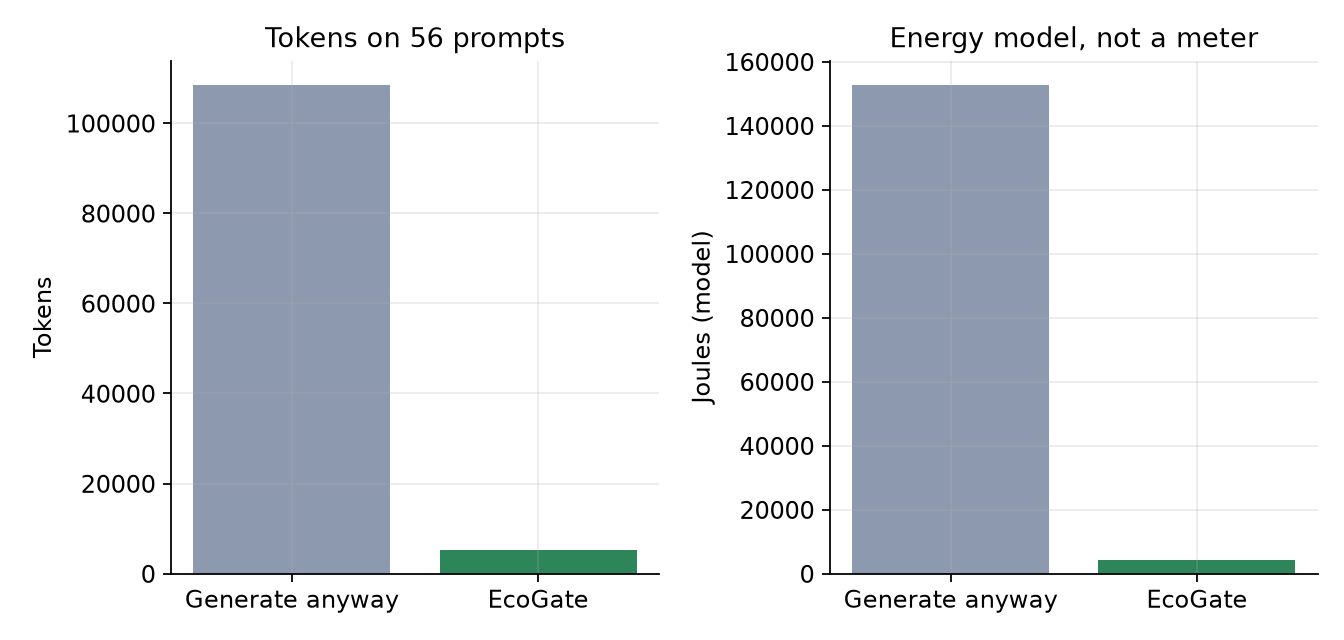
\includegraphics[width=\columnwidth]{ecogate_cost.png}
\caption{Withdrawn. Formula weights, not measured energy. Not a result of this paper.}
\label{fig:cost}
\end{figure}

Figure~\ref{fig:route} is a count of an earlier routing script: 51 prompts left on the local screen, 5 assigned a diagnostic call, 0 answered directly. It is a decision histogram from that script. It is not Table~\ref{tab:base} and not Fig.~\ref{fig:tokens}.

\begin{figure}[!t]
\centering
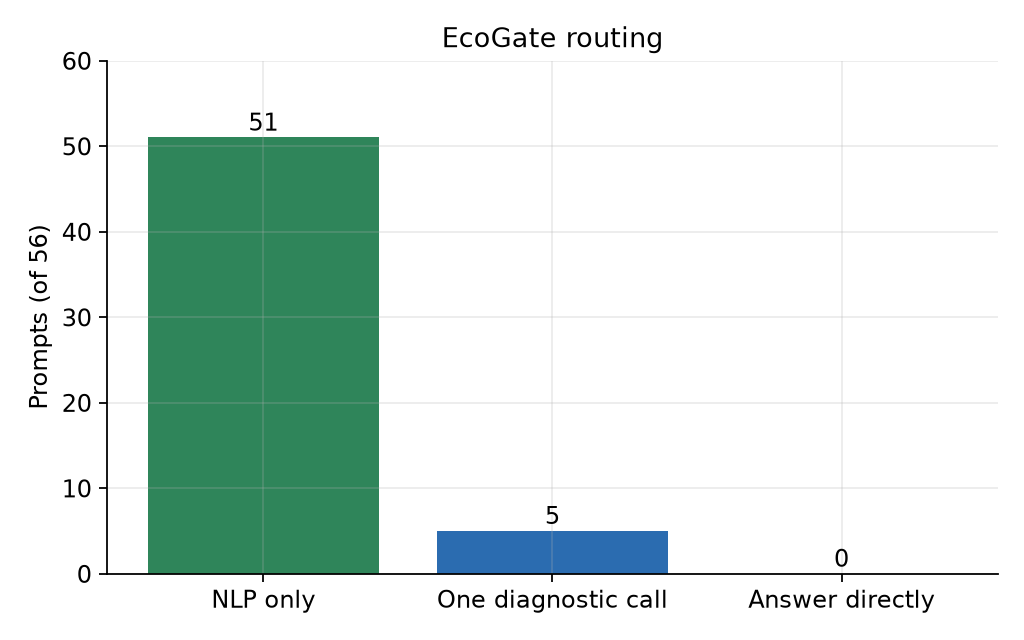
\includegraphics[width=\columnwidth]{ecogate_routing.png}
\caption{Earlier routing counts on 56 prompts. Not the specification test.}
\label{fig:route}
\end{figure}

\begin{thebibliography}{6}

\bibitem{min-etal-2020-ambigqa}
S.~Min, J.~Michael, H.~Hajishirzi, and L.~Zettlemoyer, ``{A}mbig{QA}: Answering ambiguous open-domain questions,'' in \emph{Proc.\ Empirical Methods Natural Lang.\ Process.}, 2020, pp.~5783--5797.

\bibitem{rao-daume-iii-2018-learning}
S.~Rao and H.~Daum\'e~III, ``Learning to ask good questions: Ranking clarification questions using neural expected value of perfect information,'' in \emph{Proc.\ 56th Annu.\ Meeting Assoc.\ Comput.\ Linguistics}, 2018, pp.~2737--2746.

\bibitem{zhang-choi-2025-clarify}
M.~J.~Zhang and E.~Choi, ``Clarify when necessary: Resolving ambiguity through interaction with {LM}s,'' in \emph{Findings Assoc.\ Comput.\ Linguistics: NAACL}, 2025, pp.~5541--5558.

\bibitem{kuhn-etal-2023-semantic}
L.~Kuhn, Y.~Gal, and S.~Farquhar, ``Semantic uncertainty: Linguistic invariances for uncertainty estimation in natural language generation,'' in \emph{Proc.\ Int.\ Conf.\ Learn.\ Representations}, 2023.

\bibitem{nahum-etal-2026-answers}
O.~Nahum, N.~Nayman, J.~Fhima, A.~Zolfi, J.~Levy, S.~Mazor, and P.~Favaro, ``From answers to interpretations: Rethinking ambiguity-induced aleatoric uncertainty estimation in {LLM}s,'' in \emph{Findings Assoc.\ Comput.\ Linguistics: EMNLP}, 2026.

\bibitem{chen-etal-2024-frugalgpt}
L.~Chen, M.~Zaharia, and J.~Zou, ``{F}rugal{GPT}: How to use large language models while reducing cost and improving performance,'' \emph{Trans.\ Mach.\ Learn.\ Res.}, 2024.

\end{thebibliography}

\end{document}
